\chapter{Marco Teórico y Estado del Arte}\label{chap:MarcoT}

En este capítulo se deben detallar y explicar los conceptos teóricos que sirven como base para comprender el trabajo desarrollado en la tesis. Es importante incluir únicamente los conceptos efectivamente utilizados, evitando conceptos tangenciales que no tienen aplicación directa en la tesis. Asimismo, es importante distinguir entre los conceptos básicos que el lector ya debería dominar y aquellos que realmente requieren ser explicados. Por ejemplo, explicar la ley de Ohm no debería ser necesario en una tesis de ingeniería eléctrica.

En el proceso de desarrollar los conceptos teóricos, es útil incluir figuras que ilustren los conceptos mencionados. Estas figuras tienen ciertas restricciones de formato, entre ellas: el texto que contengan debe tener un tamaño legible, su leyenda debe estar ubicada debajo de la figura, contener punto final y estar en el mismo idioma que el resto del documento. Además, las figuras no son parte del texto, y por tanto deben ser referenciadas en el texto antes de su aparición; preferentemente, deben aparecer en la misma página que su primera referencia o en la página siguiente.

Está permitido adaptar o inspirarse en figuras de otros textos, siempre y cuando se referencie claramente su procedencia en la leyenda, usando ``extraído de...'' o ``adaptado de...'' según sea el caso. La referencia debe aparecer en la leyenda del texto, pero no en la leyenda que se muestra en el índice, ya que incluirla allí puede alterar el orden de las referencias, las cuales deben enumerarse en orden de aparición en el texto. Para ello se puede utilizar el comando \texttt{\textbackslash mycaption\{Leyenda en texto\}\{Leyenda del índice\}}. Se incluyen ejemplos en las figuras \ref{img:Extraido} y \ref{img:Adaptado}. Si la figura es de producción propia, no se debe incluir ninguna indicación adicional en la leyenda; es decir, no se debe agregar ``Elaboración propia'' ni ninguna mención equivalente.

\begin{figure}[h]
    \centerline{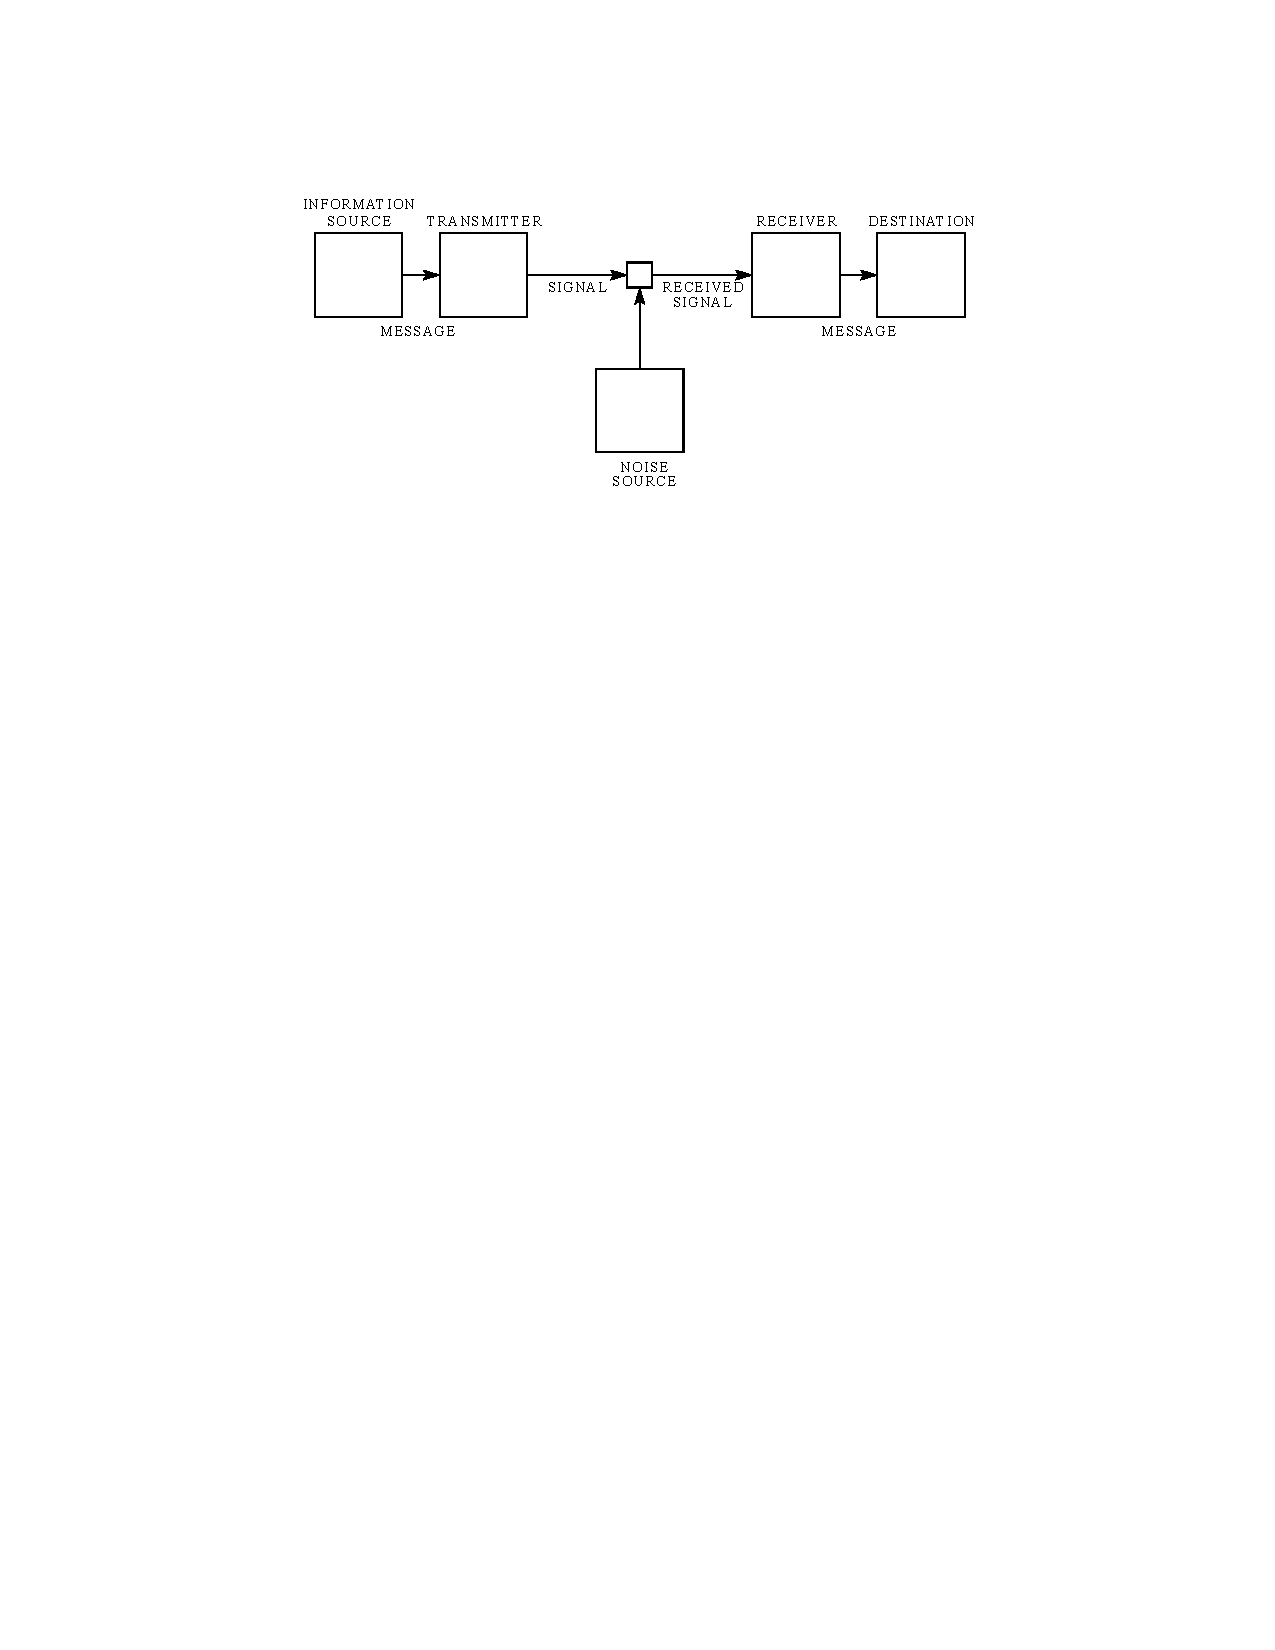
\includegraphics[width=0.6\textwidth]{Figuras/Marco_Teorico/Shannon.pdf}}
    \mycaption{Diagrama de bloques de un sistema de comunicaciones.}{Diagrama de bloques de un sistema de comunicaciones. Extraído de \cite{Shannon1948}.}
    \label{img:Extraido}
\end{figure}

\begin{figure}[h]
    \centering
    \shorthandoff{>}
    \begin{tikzpicture}[
    >=Stealth,
    block/.style={
        rectangle,
        draw=black,
        thick,
        minimum width=2.4cm,
        minimum height=1.0cm,
        align=center,
        font=\small
    },
    node distance=0.8cm
]
 
\node[block] (fuente)     {Fuente};
\node[block, right=of fuente]  (transmisor) {Transmisor};
\node[block, right=of transmisor] (canal)   {Canal};
\node[block, right=of canal]   (receptor)   {Receptor};
\node[block, right=of receptor] (destino)   {Destino};
\node[block, below=1.2cm of canal] (ruido)  {Ruido};
 
\draw[->, thick] (fuente)     -- (transmisor);
\draw[->, thick] (transmisor) -- (canal);
\draw[->, thick] (canal)      -- (receptor);
\draw[->, thick] (receptor)   -- (destino);
\draw[->, thick] (ruido)      -- (canal);
 
\end{tikzpicture}
    \shorthandon{>}
    \mycaption{Diagrama de bloques de un sistema de comunicaciones.}{Diagrama de bloques de un sistema de comunicaciones. Adaptado de \cite{Shannon1948}.}
    \label{img:Adaptado}
\end{figure}

También se deben incluir las ecuaciones que serán utilizadas en la explicación de los conceptos o en otras partes del texto, como en la metodología o en el análisis de resultados. Cabe considerar que las ecuaciones forman parte del texto y, por tanto, deben llevar la puntuación que corresponda, ya sea punto o coma. Para introducir una ecuación, se recomienda el uso de dos puntos (:), aunque cualquier otra convención es aceptable siempre que se mantenga de forma consistente a lo largo de todo el documento. En el siguiente párrafo se ejemplifica el uso correcto.

La ley de Ohm establece la relación entre el voltaje, la corriente y la resistencia en un circuito eléctrico. Dicha relación se expresa como:
\begin{equation}
    V = IR,
    \label{eq:ohm}
\end{equation}
donde $V$ es el voltaje medido en volts, $I$ es la corriente medida en amperes y $R$ es la resistencia medida en ohms. A partir de esta expresión es posible despejar cualquiera de las tres magnitudes, por ejemplo:
\begin{equation}
    I = \frac{V}{R}.
    \label{eq:ohm_despejada}
\end{equation}

Es importante mantener una notación consistente a lo largo de todo el documento. Cada variable o símbolo debe ser definido la primera vez que aparece en el texto, tal como se hizo con $V$, $I$ y $R$ en el ejemplo anterior. 

\section{Estado del Arte}
Se debe incluir una revisión del estado del arte para respaldar la novedad del trabajo. Si esta revisión fuese de gran extensión, se puede crear un capítulo separado para ella. Se recomienda describir cada referencia de forma individual, por ejemplo: ``En \cite{Shannon1948} se propone...'', ``En \cite{Shannon1948} los autores...''. En cuanto a la selección de referencias, se debe priorizar las fuentes más relevantes para el área de investigación. En la mayoría de los casos esto corresponde a artículos publicados en revistas científicas indexadas, aunque dependiendo del contexto otras fuentes pueden ser igualmente relevantes, como artículos de conferencias o reportes técnicos de organismos de referencia en el área. En cualquier caso, se debe preferir referencias recientes, idealmente de los últimos cinco años, salvo que se trate de trabajos fundacionales. Para finalizar, se recomienda incluir una tabla resumen de todos estos trabajos que incluya además esta tesis, de manera de visualizar claramente su novedad en el área. Un ejemplo de esto se muestra en la tabla~\ref{tab:SoTA}.

\begin{table}[h]
    \centering
    \caption{Resumen del estado del arte. \label{tab:SoTA}}
    \begin{tabular}{|l|c|c|c|c|}
        \hline
        \textbf{Referencia} & \textbf{Prop. 1} & \textbf{Prop. 2} & \textbf{Prop. 3} & \textbf{Métrica} \\
        \hline
        Autor A \cite{Shannon1948} & A & A & B & $x_1$ \\
        Autor B \cite{berrou1993} & B & A & A & $x_2$ \\
        Autor C \cite{haykin2001} & A & B & A & $x_3$ \\
        Autor D \cite{ieee80211_2020} & B & B & B & $x_4$ \\
        \hline
        \textbf{Esta tesis}        & \textbf{A} & \textbf{B} & \textbf{B} & $\mathbf{x_5}$ \\
        \hline
    \end{tabular}
\end{table}

Sobre las tablas, aplican las mismas reglas que para las figuras: las leyendas deben tener punto final y, si la tabla es extraída o adaptada de alguna referencia, se debe incluir esa información en la leyenda. Las tablas no forman parte del texto y deben ser referenciadas antes de su aparición. Sin embargo, hay un detalle importante: a diferencia de las figuras, la leyenda de las tablas va encima y no debajo. Es importante no exceder los márgenes del documento. Si una tabla es demasiado ancha, se permite rotarla 90° utilizando el entorno \texttt{sidewaystable} del paquete \texttt{rotating}.